%% bare_conf.tex
%% V1.4b
%% 2015/08/26
%% by Michael Shell
%% See:
%% http://www.michaelshell.org/
%% for current contact information.
%%
%% This is a skeleton file demonstrating the use of IEEEtran.cls
%% (requires IEEEtran.cls version 1.8b or later) with an IEEE
%% conference paper.
%%
%% Support sites:
%% http://www.michaelshell.org/tex/ieeetran/
%% http://www.ctan.org/pkg/ieeetran
%% and
%% http://www.ieee.org/

%%*************************************************************************
%% Legal Notice:
%% This code is offered as-is without any warranty either expressed or
%% implied; without even the implied warranty of MERCHANTABILITY or
%% FITNESS FOR A PARTICULAR PURPOSE! 
%% User assumes all risk.
%% In no event shall the IEEE or any contributor to this code be liable for
%% any damages or losses, including, but not limited to, incidental,
%% consequential, or any other damages, resulting from the use or misuse
%% of any information contained here.
%%
%% All comments are the opinions of their respective authors and are not
%% necessarily endorsed by the IEEE.
%%
%% This work is distributed under the LaTeX Project Public License (LPPL)
%% ( http://www.latex-project.org/ ) version 1.3, and may be freely used,
%% distributed and modified. A copy of the LPPL, version 1.3, is included
%% in the base LaTeX documentation of all distributions of LaTeX released
%% 2003/12/01 or later.
%% Retain all contribution notices and credits.
%% ** Modified files should be clearly indicated as such, including  **
%% ** renaming them and changing author support contact information. **
%%*************************************************************************


% *** Authors should verify (and, if needed, correct) their LaTeX system  ***
% *** with the testflow diagnostic prior to trusting their LaTeX platform ***
% *** with production work. The IEEE's font choices and paper sizes can   ***
% *** trigger bugs that do not appear when using other class files.       ***                          ***
% The testflow support page is at:
% http://www.michaelshell.org/tex/testflow/



\documentclass[conference]{IEEEtran}
% Some Computer Society conferences also require the compsoc mode option,
% but others use the standard conference format.
%
% If IEEEtran.cls has not been installed into the LaTeX system files,
% manually specify the path to it like:
% \documentclass[conference]{../sty/IEEEtran}

\usepackage[brazilian]{babel}
\usepackage[utf8]{inputenc}
\usepackage[T1]{fontenc}
%\usepackage{dirtytalk}


% Some very useful LaTeX packages include:
% (uncomment the ones you want to load)


% *** MISC UTILITY PACKAGES ***
%
%\usepackage{ifpdf}
% Heiko Oberdiek's ifpdf.sty is very useful if you need conditional
% compilation based on whether the output is pdf or dvi.
% usage:
% \ifpdf
%   % pdf code
% \else
%   % dvi code
% \fi
% The latest version of ifpdf.sty can be obtained from:
% http://www.ctan.org/pkg/ifpdf
% Also, note that IEEEtran.cls V1.7 and later provides a builtin
% \ifCLASSINFOpdf conditional that works the same way.
% When switching from latex to pdflatex and vice-versa, the compiler may
% have to be run twice to clear warning/error messages.






% *** CITATION PACKAGES ***
%
%\usepackage{cite}
% cite.sty was written by Donald Arseneau
% V1.6 and later of IEEEtran pre-defines the format of the cite.sty package
% \cite{} output to follow that of the IEEE. Loading the cite package will
% result in citation numbers being automatically sorted and properly
% "compressed/ranged". e.g., [1], [9], [2], [7], [5], [6] without using
% cite.sty will become [1], [2], [5]--[7], [9] using cite.sty. cite.sty's
% \cite will automatically add leading space, if needed. Use cite.sty's
% noadjust option (cite.sty V3.8 and later) if you want to turn this off
% such as if a citation ever needs to be enclosed in parenthesis.
% cite.sty is already installed on most LaTeX systems. Be sure and use
% version 5.0 (2009-03-20) and later if using hyperref.sty.
% The latest version can be obtained at:
% http://www.ctan.org/pkg/cite
% The documentation is contained in the cite.sty file itself.






% *** GRAPHICS RELATED PACKAGES ***
%
\ifCLASSINFOpdf
   \usepackage[pdftex]{graphicx}
  % declare the path(s) where your graphic files are
   \graphicspath{{../pdf/}{../jpeg/}{./}}
  % and their extensions so you won't have to specify these with
  % every instance of \includegraphics
   \DeclareGraphicsExtensions{.pdf,.jpeg,.png}
\else
  % or other class option (dvipsone, dvipdf, if not using dvips). graphicx
  % will default to the driver specified in the system graphics.cfg if no
  % driver is specified.
   \usepackage[dvips]{graphicx}
  % declare the path(s) where your graphic files are
   \graphicspath{{../eps/}}
  % and their extensions so you won't have to specify these with
  % every instance of \includegraphics
   \DeclareGraphicsExtensions{.eps}
\fi
% graphicx was written by David Carlisle and Sebastian Rahtz. It is
% required if you want graphics, photos, etc. graphicx.sty is already
% installed on most LaTeX systems. The latest version and documentation
% can be obtained at: 
% http://www.ctan.org/pkg/graphicx
% Another good source of documentation is "Using Imported Graphics in
% LaTeX2e" by Keith Reckdahl which can be found at:
% http://www.ctan.org/pkg/epslatex
%
% latex, and pdflatex in dvi mode, support graphics in encapsulated
% postscript (.eps) format. pdflatex in pdf mode supports graphics
% in .pdf, .jpeg, .png and .mps (metapost) formats. Users should ensure
% that all non-photo figures use a vector format (.eps, .pdf, .mps) and
% not a bitmapped formats (.jpeg, .png). The IEEE frowns on bitmapped formats
% which can result in "jaggedy"/blurry rendering of lines and letters as
% well as large increases in file sizes.
%
% You can find documentation about the pdfTeX application at:
% http://www.tug.org/applications/pdftex





% *** MATH PACKAGES ***
%
%\usepackage{amsmath}
% A popular package from the American Mathematical Society that provides
% many useful and powerful commands for dealing with mathematics.
%
% Note that the amsmath package sets \interdisplaylinepenalty to 10000
% thus preventing page breaks from occurring within multiline equations. Use:
%\interdisplaylinepenalty=2500
% after loading amsmath to restore such page breaks as IEEEtran.cls normally
% does. amsmath.sty is already installed on most LaTeX systems. The latest
% version and documentation can be obtained at:
% http://www.ctan.org/pkg/amsmath





% *** SPECIALIZED LIST PACKAGES ***
%
%\usepackage{algorithmic}
% algorithmic.sty was written by Peter Williams and Rogerio Brito.
% This package provides an algorithmic environment fo describing algorithms.
% You can use the algorithmic environment in-text or within a figure
% environment to provide for a floating algorithm. Do NOT use the algorithm
% floating environment provided by algorithm.sty (by the same authors) or
% algorithm2e.sty (by Christophe Fiorio) as the IEEE does not use dedicated
% algorithm float types and packages that provide these will not provide
% correct IEEE style captions. The latest version and documentation of
% algorithmic.sty can be obtained at:
% http://www.ctan.org/pkg/algorithms
% Also of interest may be the (relatively newer and more customizable)
% algorithmicx.sty package by Szasz Janos:
% http://www.ctan.org/pkg/algorithmicx




% *** ALIGNMENT PACKAGES ***
%
%\usepackage{array}
% Frank Mittelbach's and David Carlisle's array.sty patches and improves
% the standard LaTeX2e array and tabular environments to provide better
% appearance and additional user controls. As the default LaTeX2e table
% generation code is lacking to the point of almost being broken with
% respect to the quality of the end results, all users are strongly
% advised to use an enhanced (at the very least that provided by array.sty)
% set of table tools. array.sty is already installed on most systems. The
% latest version and documentation can be obtained at:
% http://www.ctan.org/pkg/array


% IEEEtran contains the IEEEeqnarray family of commands that can be used to
% generate multiline equations as well as matrices, tables, etc., of high
% quality.




% *** SUBFIGURE PACKAGES ***
%\ifCLASSOPTIONcompsoc
%  \usepackage[caption=false,font=normalsize,labelfont=sf,textfont=sf]{subfig}
%\else
%  \usepackage[caption=false,font=footnotesize]{subfig}
%\fi
% subfig.sty, written by Steven Douglas Cochran, is the modern replacement
% for subfigure.sty, the latter of which is no longer maintained and is
% incompatible with some LaTeX packages including fixltx2e. However,
% subfig.sty requires and automatically loads Axel Sommerfeldt's caption.sty
% which will override IEEEtran.cls' handling of captions and this will result
% in non-IEEE style figure/table captions. To prevent this problem, be sure
% and invoke subfig.sty's "caption=false" package option (available since
% subfig.sty version 1.3, 2005/06/28) as this is will preserve IEEEtran.cls
% handling of captions.
% Note that the Computer Society format requires a larger sans serif font
% than the serif footnote size font used in traditional IEEE formatting
% and thus the need to invoke different subfig.sty package options depending
% on whether compsoc mode has been enabled.
%
% The latest version and documentation of subfig.sty can be obtained at:
% http://www.ctan.org/pkg/subfig




% *** FLOAT PACKAGES ***
%
%\usepackage{fixltx2e}
% fixltx2e, the successor to the earlier fix2col.sty, was written by
% Frank Mittelbach and David Carlisle. This package corrects a few problems
% in the LaTeX2e kernel, the most notable of which is that in current
% LaTeX2e releases, the ordering of single and double column floats is not
% guaranteed to be preserved. Thus, an unpatched LaTeX2e can allow a
% single column figure to be placed prior to an earlier double column
% figure.
% Be aware that LaTeX2e kernels dated 2015 and later have fixltx2e.sty's
% corrections already built into the system in which case a warning will
% be issued if an attempt is made to load fixltx2e.sty as it is no longer
% needed.
% The latest version and documentation can be found at:
% http://www.ctan.org/pkg/fixltx2e


%\usepackage{stfloats}
% stfloats.sty was written by Sigitas Tolusis. This package gives LaTeX2e
% the ability to do double column floats at the bottom of the page as well
% as the top. (e.g., "\begin{figure*}[!b]" is not normally possible in
% LaTeX2e). It also provides a command:
%\fnbelowfloat
% to enable the placement of footnotes below bottom floats (the standard
% LaTeX2e kernel puts them above bottom floats). This is an invasive package
% which rewrites many portions of the LaTeX2e float routines. It may not work
% with other packages that modify the LaTeX2e float routines. The latest
% version and documentation can be obtained at:
% http://www.ctan.org/pkg/stfloats
% Do not use the stfloats baselinefloat ability as the IEEE does not allow
% \baselineskip to stretch. Authors submitting work to the IEEE should note
% that the IEEE rarely uses double column equations and that authors should try
% to avoid such use. Do not be tempted to use the cuted.sty or midfloat.sty
% packages (also by Sigitas Tolusis) as the IEEE does not format its papers in
% such ways.
% Do not attempt to use stfloats with fixltx2e as they are incompatible.
% Instead, use Morten Hogholm'a dblfloatfix which combines the features
% of both fixltx2e and stfloats:
%
% \usepackage{dblfloatfix}
% The latest version can be found at:
% http://www.ctan.org/pkg/dblfloatfix




% *** PDF, URL AND HYPERLINK PACKAGES ***
%
%\usepackage{url}
% url.sty was written by Donald Arseneau. It provides better support for
% handling and breaking URLs. url.sty is already installed on most LaTeX
% systems. The latest version and documentation can be obtained at:
% http://www.ctan.org/pkg/url
% Basically, \url{my_url_here}.




% *** Do not adjust lengths that control margins, column widths, etc. ***
% *** Do not use packages that alter fonts (such as pslatex).         ***
% There should be no need to do such things with IEEEtran.cls V1.6 and later.
% (Unless specifically asked to do so by the journal or conference you plan
% to submit to, of course. )


% correct bad hyphenation here
\hyphenation{op-tical net-works semi-conduc-tor}


\begin{document}
%
% paper title
% Titles are generally capitalized except for words such as a, an, and, as,
% at, but, by, for, in, nor, of, on, or, the, to and up, which are usually
% not capitalized unless they are the first or last word of the title.
% Linebreaks \\ can be used within to get better formatting as desired.
% Do not put math or special symbols in the title.
\title{A Origem da Internet}


% author names and affiliations
% use a multiple column layout for up to three different
% affiliations
\author{\IEEEauthorblockN{Pedro Cunial Campos}
	\IEEEauthorblockA{Insper\\
		São Paulo, SP\\
		pedrocc4@al.insper.edu.br}}

% conference papers do not typically use \thanks and this command
% is locked out in conference mode. If really needed, such as for
% the acknowledgment of grants, issue a \IEEEoverridecommandlockouts
% after \documentclass

% for over three affiliations, or if they all won't fit within the width
% of the page, use this alternative format:
% 
%\author{\IEEEauthorblockN{Michael Shell\IEEEauthorrefmark{1},
%Homer Simpson\IEEEauthorrefmark{2},
%James Kirk\IEEEauthorrefmark{3}, 
%Montgomery Scott\IEEEauthorrefmark{3} and
%Eldon Tyrell\IEEEauthorrefmark{4}}
%\IEEEauthorblockA{\IEEEauthorrefmark{1}School of Electrical and Computer Engineering\\
%Georgia Institute of Technology,
%Atlanta, Georgia 30332--0250\\ Email: see http://www.michaelshell.org/contact.html}
%\IEEEauthorblockA{\IEEEauthorrefmark{2}Twentieth Century Fox, Springfield, USA\\
%Email: homer@thesimpsons.com}
%\IEEEauthorblockA{\IEEEauthorrefmark{3}Starfleet Academy, San Francisco, California 96678-2391\\
%Telephone: (800) 555--1212, Fax: (888) 555--1212}
%\IEEEauthorblockA{\IEEEauthorrefmark{4}Tyrell Inc., 123 Replicant Street, Los Angeles, California 90210--4321}}




% use for special paper notices
%\IEEEspecialpapernotice{(Invited Paper)}




% make the title area
\maketitle

% As a general rule, do not put math, special symbols or citations
% in the abstract
\begin{abstract}
  
  Explorando temáticas sobre RFC, modelo TCP/IP e a história pré, pós e durante a ARPANET, este artigo busca descrever o processo da criação da Internet em seu primórdio e seu desenvolvimento e evolução, traçando paralelos com o que conhecemos hoje por internet e almejando compreender os motivos pelos quais os atuais formatos e protocolos de comunicação são utilizados, sob a óptica das telecomunicações.
\end{abstract}
% no keyword




% For peer review papers, you can put extra information on the cover
% page as needed:
% \ifCLASSOPTIONpeerreview
% \begin{center} \bfseries EDICS Category: 3-BBND \end{center}
% \fi
%
% For peerreview papers, this IEEEtran command inserts a page break and
% creates the second title. It will be ignored for other modes.
\IEEEpeerreviewmaketitle





%% \subsection{Definindo violencia}
%% Subsection text here.


%% \subsubsection{Subsubsection Heading Here}
%% Subsubsection text here.


% An example of a floating figure using the graphicx package.
% Note that \label must occur AFTER (or within) \caption.
% For figures, \caption should occur after the \includegraphics.
% Note that IEEEtran v1.7 and later has special internal code that
% is designed to preserve the operation of \label within \caption
% even when the captionsoff option is in effect. However, because
% of issues like this, it may be the safest practice to put all your
% \label just after \caption rather than within \caption{}.
%
% Reminder: the "draftcls" or "draftclsnofoot", not "draft", class
% option should be used if it is desired that the figures are to be
% displayed while in draft mode.
%
%\begin{figure}[!t]
%\centering
%\includegraphics[width=2.5in]{myfigure}
% where an .eps filename suffix will be assumed under latex, 
% and a .pdf suffix will be assumed for pdflatex; or what has been declared
% via \DeclareGraphicsExtensions.
%\caption{Simulation results for the network.}
%\label{fig_sim}
%\end{figure}

% Note that the IEEE typically puts floats only at the top, even when this
% results in a large percentage of a column being occupied by floats.


% An example of a double column floating figure using two subfigures.
% (The subfig.sty package must be loaded for this to work.)
% The subfigure \label commands are set within each subfloat command,
% and the \label for the overall figure must come after \caption.
% \hfil is used as a separator to get equal spacing.
% Watch out that the combined width of all the subfigures on a 
% line do not exceed the text width or a line break will occur.
%
%\begin{figure*}[!t]
%\centering
%\subfloat[Case I]{\includegraphics[width=2.5in]{box}%
%\label{fig_first_case}}
%\hfil
%\subfloat[Case II]{\includegraphics[width=2.5in]{box}%
%\label{fig_second_case}}
%\caption{Simulation results for the network.}
%\label{fig_sim}
%\end{figure*}
%
% Note that often IEEE papers with subfigures do not employ subfigure
% captions (using the optional argument to \subfloat[]), but instead will
% reference/describe all of them (a), (b), etc., within the main caption.
% Be aware that for subfig.sty to generate the (a), (b), etc., subfigure
% labels, the optional argument to \subfloat must be present. If a
% subcaption is not desired, just leave its contents blank,
% e.g., \subfloat[].


% An example of a floating table. Note that, for IEEE style tables, the
% \caption command should come BEFORE the table and, given that table
% captions serve much like titles, are usually capitalized except for words
% such as a, an, and, as, at, but, by, for, in, nor, of, on, or, the, to
% and up, which are usually not capitalized unless they are the first or
% last word of the caption. Table text will default to \footnotesize as
% the IEEE normally uses this smaller font for tables.
% The \label must come after \caption as always.
%
%\begin{table}[!t]
%% increase table row spacing, adjust to taste
%\renewcommand{\arraystretch}{1.3}
% if using array.sty, it might be a good idea to tweak the value of
% \extrarowheight as needed to properly center the text within the cells
%\caption{An Example of a Table}
%\label{table_example}
%\centering
%% Some packages, such as MDW tools, offer better commands for making tables
%% than the plain LaTeX2e tabular which is used here.
%\begin{tabular}{|c||c|}
%\hline
%One & Two\\
%\hline
%Three & Four\\
%\hline
%\end{tabular}
%\end{table}


% Note that the IEEE does not put floats in the very first column
% - or typically anywhere on the first page for that matter. Also,
% in-text middle ("here") positioning is typically not used, but it
% is allowed and encouraged for Computer Society conferences (but
% not Computer Society journals). Most IEEE journals/conferences use
% top floats exclusively. 
% Note that, LaTeX2e, unlike IEEE journals/conferences, places
% footnotes above bottom floats. This can be corrected via the
% \fnbelowfloat command of the stfloats package.

\section{Introdução}
% no \IEEEPARstart
	% Neste artigo pretendo dissecar os passos iniciais dos aspectos de telecomunicação da Internet, desdo seu processo inicial de ideação (em 1966), enquanto ainda era um projeto fechado, até a sua abertura ao público e revisões baseadas em seus primeiros dias, chegando ao início da década de 1980.
  Em 1962, nos Estados Unidos, a Agência de Projetos de Pesquisa Avançada (Advanced Research Projects Agency -- ARPA) criaria um novo
  braço, o Escritório de Técnicas de Processamento de Informações (Information Processing Technical Office -- IPTO), o qual se
  tornaria enorme referência em estudos de ciência da computação nos Estados
  Unidos durante seu tempo~\cite{fromarpanet}, enriquecendo tremendamente os
  estudos em áreas como a de processamento de gráficos, inteligência artificial e
  multitasking.

  Mas fora em 1966, quando Robert Taylor iniciou seus estudos em redes e assumira a liderança do IPTO que a Internet seria idealizada pela primeira vez. A proposta de Taylor consistia em suprir duas necessidades: a redução de custos em computação pelo compartilhamento de computadores por contratantes ao redor do país e o avanço na transferência de informações entre máquinas à distância~\cite{fromarpanet}.

\section{Primeiros passos}
%	Neste parágrafo pretendo explicar os processos iniciais de ideação, anteriores às primeiras versões da mesma. Pretendo basear este parágrafo fortemente na descrição do período pelo artigo "From ARPANET to Internet"~\cite{fromarpanet}, prendendo-me aos períodos anteriores ao ano de 1969, quando a primeira versão da ARPANET for publicada.
Dado a tensão entre potências que definia a Guerra Fria, os estudos de Taylor e sua equipe mantiveram-se sigilosos,mas que tornar-se-iam, cada vez mais, de extremo interesse para o Estado norte-americano, o qual investiria em peso no projeto.
  \begin{quote}
    Quando o Departamento de Defesa (Department of Defense -- DOD) emitiu um contrato de \$19.800 em
    6 de Dezembro de 1967 sob o proposito de estudar "design e especificação de uma
    rede de computadores", o mundo não se deu conta do que estava prestes à
    acontecer. Fora neste estudo de quatro meses que surgiria a primeira versão
    da ARPANET (ARPA NETwork)~\cite{internethistory}. 
  \end{quote}

  Pela confidencialidade do projeto, não se sabe exatamente o que ocorrera de
  fato nestes primeiros anos, apenas que em 1968 mais \$63.000 seriam investidos, e que sua segunda versão seria liberada em 1969,
   "com uma revolução nas comunicações pelas palavras
    \emph{log in}"~\cite{fromarpanet}, representando um primeiro sinal de uso, assinatura e autenticação pessoal para as comunicações nesta rede.
	
% \section{O Caos}
	% Pretendo descrever processos associados à criação e resposta às primeiras versões da ARPANET. Imagino que eu vá bater com o conceito de RFC já na seção anterior, mas se não for o caso, certamente será descrito nesta seção.
	
	% Acredito que tenho muito para extrair do "Internet History"~\cite{internethistory}, mas principalmente do "The Framing Years"~\cite{framingyears}, no qual as primeiras seções são especialmente uteis.

  Fora somente nessa segunda versão que o mundo acadêmico entraria em contato
  com o invento, conectando computadores da UCLA, UC-Santa Barbara, Stanford e
  da Universidade de Utah~\cite{fromarpanet}.

  No entanto, ainda não existiam padrões no formato das
  comunicações, gerando um verdadeiro caos, onde os destinatários das mensagens nem sempre conseguiam decodificar o sinal recebido, ou, quando conseguiam, não eram capazes de decifrar seu conteúdo, dada as diferentes maneiras pelas quais os sinais eram codificados ao serem enviados por diferentes emissores.%

  Buscando solucionar o problema, Steve Crocker, estudante da UCLA que trabalhara no desenvolvimento das comunicações da ARPANET desde sua primeira abertura à sua universidade, criaria o padrão dos Request For Comments
  (RFC) em 1969, que seriam mantidos pelo "Grupo de Trabalho sobre Redes" (do qual Crocker fora parte crítica para criação) e atualmente mantidos pela Internet Engineering Task Force (IETF), como documentado no RFC 100:

  \begin{quote}

    Sob a pressão de ``colocar as coisa para funcionar'' (...) definimos o
    primeiro conjunto de protocolos, incluindo somente o \emph{Telnet} e o
    \emph{File Transfer Protocol (FTP)}. Em Dezembro de 1969 nos encontramos com
    Larry Roberts \emph{(Universidade de Utah)}, com quem sofremos nossa
    primeira experiência direta com ``redirecionamento''.
    Larry deixou bem claro que nosso primeiro passo não fora grande o
    suficiente e que precisaríamos voltar aos planejamentos.~\cite{rfc100}
    
  \end{quote}
  
  A contribuição de Crocker fora de tamanha relevância que em 2002 a \emph{IEEE Internet} o atribuiria seu maior prêmio ao primeiro RFC e à Crocker pela sua contribuição para comunidade.

  Em 2011 já haviam mais de 6.200 documentos~\cite{framingyears}, que vão desda
  descrição de sistemas sociais e técnicos (RFC 2555), guias para criação de
  redes (RFC 356), ``netiqueta'' ou guias para usuários
  (RFC 1855)~\cite{framingyears}. Como
  consequência os RFCs têm sido objeto de estudos não só de cientistas da
  computação, mas também de cientistas sociais e outros profissionais de
  humanidades.

  \section{Surgimento do TCP/IP}
	% O TCP fora criado dentro da própria DARPA e inicialmente não fazia parte do padrão utilizado pela ARPANET. Nesta parte do artigo pretendo expandir dentro desta temática. Em "Framing Years"~\cite{framingyears} o autor expande um pouco no tema, mas acredito que precisarei de mais fontes para esta parte.
	
	% Dentro das fontes já utilizadas, o "Internet History"~\cite{internethistory} possui um pouco mais de conteúdo no assunto, mas nada tão profundo quanto eu gostaria.

  Motivado pelo discurso e problema de redirecionamento mostrado por Larry
  Roberts e citado no RFC 100~\cite{rfc100}, em 1973 o Transmission Control
  Protocol (TCP) fora criado~\cite{framingyears}, sob o RFC de número 604. Um
  protocolo que buscava especificar como enviar informações de um programa em um
  dado computador para outro programa em outro computador, buscando substituir o
  então padrão do NCP, o qual também fora apresentado no RFC 100:

  \begin{quote}

    Nos últimos meses, estivemos desenvolvendo um protocolo simétrico
    \emph{host-host}. À sua implementação, ainda abstrata ficou conhecida como 
    \emph{Network Control Protocol} (``NCP'' inicialmente pretendia apenas ser o
    programa dentro do Sistema Operacional que gerenciava as conexões).
    ~\cite{rfc100}
    
  \end{quote}
  
  No entanto, fora somente em conjunto com o Internet Protocol (IP, RFC 675), o
  qual buscava especificar a forma com que dados deveriam ser direcionados, que a
  ARPANET abandonaria o NCP, adotando o TCP/IP (RFC 714, junção dos dois
  protocolos TCP e IP em um só), desenvolvido por
  Vinton Cerf e Robert Kahn~\cite{fromarpanet}, como um padrão para todos os
  computadores que se conectassem nela, como documentado no RFC 801~\cite{rfc801} -- intitulado de \emph{NCP/TCP TRANSITION PLAN}, o RFC 801 busca não só argumentar à favor do modelo TCP/IP como também declarar um plano para que a transição fosse bem sucedida.
  
  Baseando-se no sucesso do TCP/IP em implementações, o documento urge pela implementação do modelo em todas as redes que ainda se comunicavam por NCP com início em primeiro de janeiro de 1982 e um prazo máximo de primeiro de janeiro  de 1983~\cite{rfc801}.
  
% \section{TCP/IP e como ele fora adotado como padrão}
% 	Aqui pretendo expandir no conceito dos RFC's iniciais e como o formato
%   original fora substituído pelo modelo TCP/IP. Sinceramente, ainda não tenho
%   muita certeza se devo explicar o conceito de IP e a união com o protocolo TCP.
%   De qualquer forma, o "Framing Years"~\cite{framingyears} fala mais sobre esta
%   transição do qe os outros artigos, por isso acredito que ele seja uma
%   referência melhor.

\section{O Email}

	Definido como "um meio para troca de mensagens digitais entre usuários de computadores", o email surgira com base na utilização do FTP para troca de mensagens~\cite{rfc561}. No entanto, a falta de padronização na escrita destes "correspondências pela rede" (Network Mail, como eram chamadas), culminou no primeiro caso no qual a Network Working Group publicaria um RFC voltado à formatação e etiqueta na comunicação entre usuários pela sua rede, o RFC 561 onde é definido a formatação de cabeçalhos destas "correspondências" (repare que na época ainda não existia o termo \emph{email}).~\cite{rfc561}
	
	No entanto, a falta de padronização nos pacotes de comunicação ainda eram um problema na época e a comunicação por \emph{Network Mail} não fugiria a esta regra. Foi com isso que em 1981 o "Simple Mail Transfer Protocol" fora criado, buscando maior eficiência e confiabilidade na transferência destes dados.~\cite{rfc788}. Um ponto à ser retomado 
	
\begin{figure}[h]
	\centering
	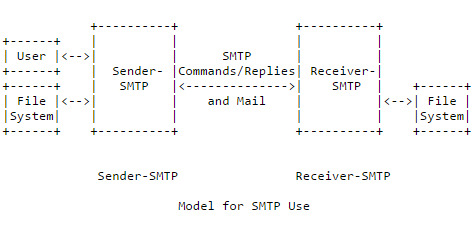
\includegraphics[width=3.1in]{smtp}
	\caption{Gráfico utilizado para ilustrar a comunicação por SMTP,
	em RFC 821.~\cite{rfc821}}
	\label{smtp_fig}
\end{figure}

	A figura acima aparece no RFC 821, com o intuito de ilustrar o processo de envio e requerimento de dados por ambas as partes participadoras da comunicação por SMTP. Repare que o SMTP-Receptor pode ou não ser o destinatário final (permitindo que dados fossem retransmitidos, ou passassem por roteadores intermediários) e que a imagem fora feita inteiramente com caracteres da tabela ASCII, os quais eram a única forma pela qual dados poderiam ser transferidos no SMTP idealizado naquele período.~\cite{rfc821}


	
\section{Da ARPANET para a Internet}
	% Com o panorama histórico já traçado, pretendo concluir meu texto trazendo algumas novidades adicionadas em RFC's mais recentes e talvez alguma provocação, como a do artigo "Two-bit Differentiated"~\cite{twobit}. 

  No final da década de 1980, a Fundação Nacional de Ciências começou a
  construir o NSFNET, um supercomputador com o intuito designar e centralizar as
  ligações de rede da ARPANET~\cite{nsfnet} -- aos que cuidam do processo de designação e
  ligação chamamos de \emph{backbone}.

  Além de ser o backbone da ARPNET, o NSFNET também servia como material de
  estudo para membros de diversas universidades, como a de Minnesota, e
  corporações, como a Bell Labs, por exemplo~\cite{nsfnet}.

  Em 1989, o NSFNET teve a velocidade do serviço do seu backbone aumentada de T1
  (1,5Mpbs) para T3 (45Mpbs), o que causaria um enorme fluxo de dados no NSFNET
  e uma responsabilidade maior do que estavam prontos para lidar, culminando no
  início de uma nova era: A era da Internet.

  \begin{quote}

    Em 1990 e 1991, o time do NSFNET fora reestruturado. Uma entidade de
    fins não lucrativos chamada Advanced Network and Services continuou provendo
    o antigo serviço de backbone (...), enquanto uma de fins lucrativos
    tornar-se-ia um desmembramento da matriz com intuito de habilitar o
    desenvolvimento comercial do projeto.~\cite{nsfnet}

  \end{quote}

  Inaugurado em 1991, o novo serviço T3 marcou o início do que conhecemos como
  Internet, já linkando mais de 3.500 redes e 16 sites em seu primeiro dia de
  funcionamento~\cite{nsfnet}.

  Ainda em Março de 1991 a Internet já transmitia 1.3 trilhões de bytes de
  informação por mês, valor que chegaria à quase 18 trilhões ao final de 1994,
  equivalente eletrônico à mover o conteúdo completo da Biblioteca do Congresso
  Americano à cada quatro meses~\cite{nsfnet}.

\section{Considerações Finais}

  \begin{quote}

    Em 1995, já estava claro que a Internet crescia drasticamente.
    NSFNET pulverizou o crescimento da Internet para todos os tipos de
    organizações. A NSF havia gasto cerca de \$30 milhões no NSFNET, assistido
    de diversos investidores externos, como a IBM e a MCI. Como resultado, 1995
    viu cerca de 100.000 redes -- tanto públicas como privadas -- em operação ao
    redor de todo o país.~\cite{nsfnet}
    
  \end{quote}

  Evidentemente que não da mesma forma que nos anos iniciais, a Internet
  continua crescendo dada a sua reduzida difusão em países ainda \emph{em
    desenvolvimento}, ao passo que o modelo TCP/IP continua sendo utilizado,
  ainda que com complementos -- como o UDP, que serve como uma espécie de
  \emph{checksum} associado ao pacote -- RFCs continuam sendo publicados até
  hoje e, ainda que em menor quantidade, continuam de extrema importância quanto
  à regulação do uso de novas tecnologias.
  

% conference papers do not normally have an appendix


% use section* for acknowledgment
% \section*{Acknowledgment}
% 	Gostaria de agradecer à todos aqueles que me apoiaram, ao stackoverflow e à minha mãe.






% trigger a \newpage just before the given reference
% number - used to balance the columns on the last page
% adjust value as needed - may need to be readjusted if
% the document is modified later
\IEEEtriggeratref{8}
% The "triggered" command can be changed if desired:
%\IEEEtriggercmd{\enlargethispage{-5in}}

% references section

% can use a bibliography generated by BibTeX as a .bbl file
% BibTeX documentation can be easily obtained at:
% http://mirror.ctan.org/biblio/bibtex/contrib/doc/
% The IEEEtran BibTeX style support page is at:
% http://www.michaelshell.org/tex/ieeetran/bibtex/
%\bibliographystyle{IEEEtran}
% argument is your BibTeX string definitions and bibliography database(s)
%\bibliography{IEEEabrv,../bib/paper}
%
% <OR> manually copy in the resultant .bbl file
% set second argument of \begin to the number of references
% (used to reserve space for the reference number labels box)

\begin{thebibliography}{1}
	
\bibitem{fromarpanet}
	A. Janet. \emph{From ARPANET to Internet: A History of ARPA-Sponsored Computer Networks, 1966 -- 1988}. \hskip 1em plus 0.5em minus 0.4em \relax University of Pennsylvania, Philadelphia, Pennsylvania, Estados Unidos da América. 1994.	

\bibitem{internethistory}
	Congressional Digest. \emph{Internet History -- from ARPNET to Broadband}.\hskip 1em plus 0.5em minus 0.4em \relax 2007.

\bibitem{framingyears}
  B. Sandra. \emph{The Framing Years: Policy Fundamentals in the Internet Design Proccess, 1969 -- 1979}.\hskip 1em plus 0.5em minus 0.4em \relax Department of Communication, University of Wisconsin, Milwaukee, Wisconsin, Estados Unidos da América. 2011.
  
\bibitem{twobit}
	K. Nichols, V. Jacobson, L. Zhang. \emph{A Two-bit Differentiated Services Architecture for the Internet}. \hskip 1em plus 0.5em minus 0.4em \relax The Internet Society. 1999.

\bibitem{rfc100}
  P. Karp. \emph{RFC 100}. \hskip 1em plus 0.5em minus
  0.4em \relax Network Working Group. 1971.

\bibitem{nsfnet}
  National Science Foundation. \emph{The Internet: changing the way we
    communicate}. \hskip 1em plus 0.5em minus 0.4em \relax Estados Unidos da
  América, 2014.
  
\bibitem{rfc801}
  J. Postel. \emph{RFC 801 -- NCP/TCP TRANSITION PLAN}. \hskip 1em plus 0.5em minus 0.4em \relax Network Working Group. 1981.

\bibitem{rfc788}
  J. Postel. \emph{RFC 788 -- SIMPLE MAIL TRANSFER PROTOCOL}. \hskip 1em plus 0.5em minus 0.4em \relax Network Working Group. 1981.
  
\bibitem{rfc561}
 A. Bhushan, K. Pogran, R. Tomlinson, J. White. \emph{RFC 561 -- Standardizing Network Mail Headers}. \hskip 1em plus 0.5em minus 0.4em \relax Network Working Group. 1973.
 
\bibitem{rfc821}
 J. Postel. \emph{RFC 821 -- SIMPLE MAIL TRANSFER PROTOCOL}. \hskip 1em plus 0.5em minus 0.4em \relax Network Working Group. 1982.
  
\bibliographystyle{IEEEtran}
%% \newcommand{\BIBdecl}{\bfseries\setlength
%%     {\itemsep}{1\baselineskip plus 0.1\baselineskip minus 0.1\baselineskip}
%% \bibliographystyle{IEEEtran}
%% \bibliography{IEEEabrv, pedrocunial-artigo.bib}

\end{thebibliography}




% that's all folks
\end{document}


